\documentclass{beamer}

\useoutertheme[subsection=false]{miniframes}
\usecolortheme{beaver}
\setbeamertemplate{navigation symbols}{}
\setbeamertemplate{footline}{}
\usepackage{graphicx}
\usepackage{url}
\usepackage{datetime}
\usepackage{tikz-cd}
\newcommand{\lectureDate}{\formatdate{16}{10}{2018}}

\setbeamertemplate{caption}
{\raggedright\insertcaption\par}
\title{MATH211: Linear Methods I}
\author{Matthew Burke}
\date{\lectureDate}
\begin{document}

\frame{\titlepage}

\begin{frame}{Lecture on \lectureDate}
  \tableofcontents
\end{frame}

\section*{Last time}
\label{sec:Last-time}

\begin{frame}{Last time}
  \begin{itemize}
  \item Lines and planes\vfill
  \item Scalar product, length and distance\vfill
  \item Orthogonality
  \end{itemize}
\end{frame}

\section{Orthogonality}

\begin{frame}
  \begin{beamercolorbox}[sep=12pt,center]{part title}
    \usebeamerfont{section title}\insertsection\par
  \end{beamercolorbox}
\end{frame}

\begin{frame}{Orthogonality}
  \begin{definition}
    Two vectors $u$ and $v$ are \emph{orthogonal} iff
    \begin{equation*}
      u\cdot v = 0
    \end{equation*}
  \end{definition}\vfill
  Note that a zero vector is orthogonal to any other vector.
\end{frame}

\begin{frame}{Orthogonal complement}
  \begin{definition}[Slightly non-standard]
    If $v$ is a vector then the \emph{orthogonal complement $v^{\perp}$} of $v$ is the set of all vectors $u$ such that $u\cdot v = 0$.
  \end{definition}\vfill
  Therefore
  \begin{itemize}
  \item If $v\neq 0\in \mathbb R^1$ then $v^{\perp} = 0$.
  \item If $v\neq 0\in \mathbb R^2$ then $v^{\perp}$ is the line perpendicular to $v$.
  \item If $v\neq 0\in \mathbb R^3$ then $v^{\perp}$ is a plane.
  \end{itemize}\vfill
  In general if $v\neq 0 \in \mathbb R^n$ then $v^{\perp}$ is a $(n-1)$-dimensional subspace.
\end{frame}

\begin{frame}{Lines via normal vector}
\begin{columns}
    \hspace{-1cm}
\column{0.4\textwidth}
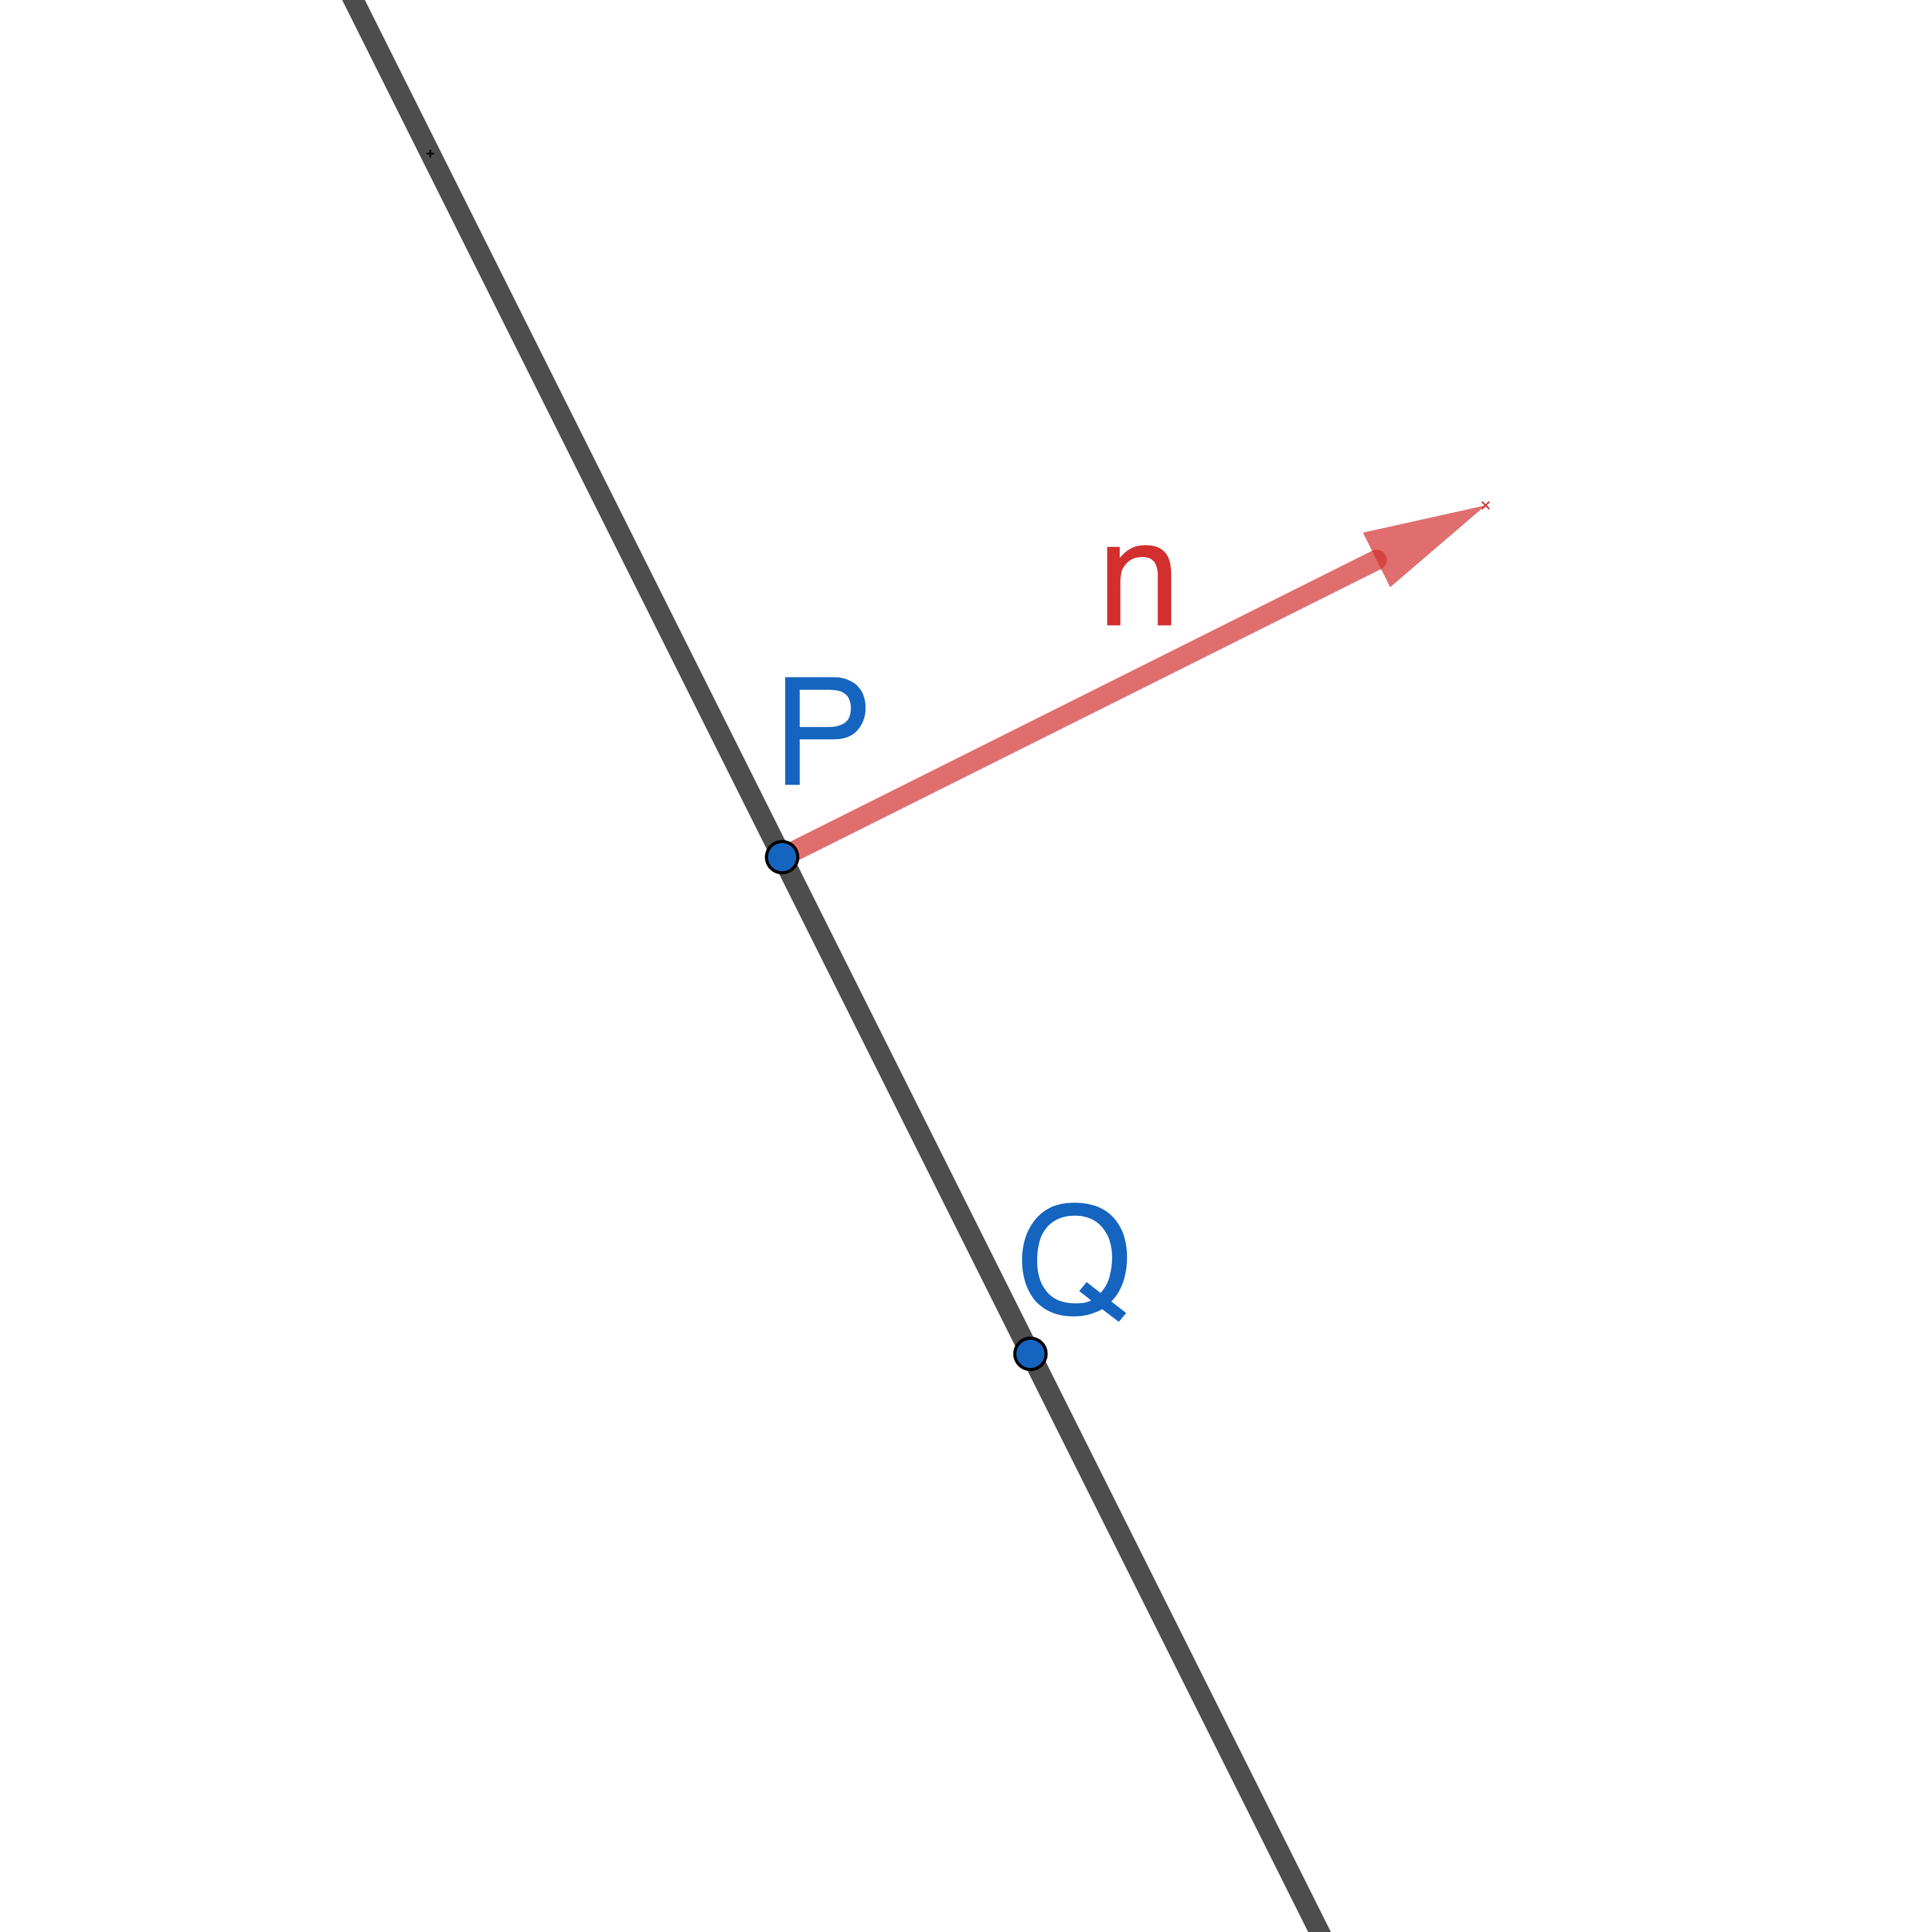
\includegraphics{2d-normal.png}
\column{0.5\textwidth}
\begin{itemize}
\item Let $P$ and $n$ be vectors in $\mathbb{R}^2$.
\item The set of points $Q$ such that $\overrightarrow{PQ}$ is orthogonal to $n$ form a line.
\item Therefore the solutions to \begin{equation*}
    n\cdot(x-P) = 0
\end{equation*}
form a line through $P$ and orthogonal to $n$.
\end{itemize}
\end{columns}
\end{frame}

\begin{frame}{Planes via normal vector}
  \begin{columns}
    \hspace{-1cm}
    \column{0.5\textwidth}
    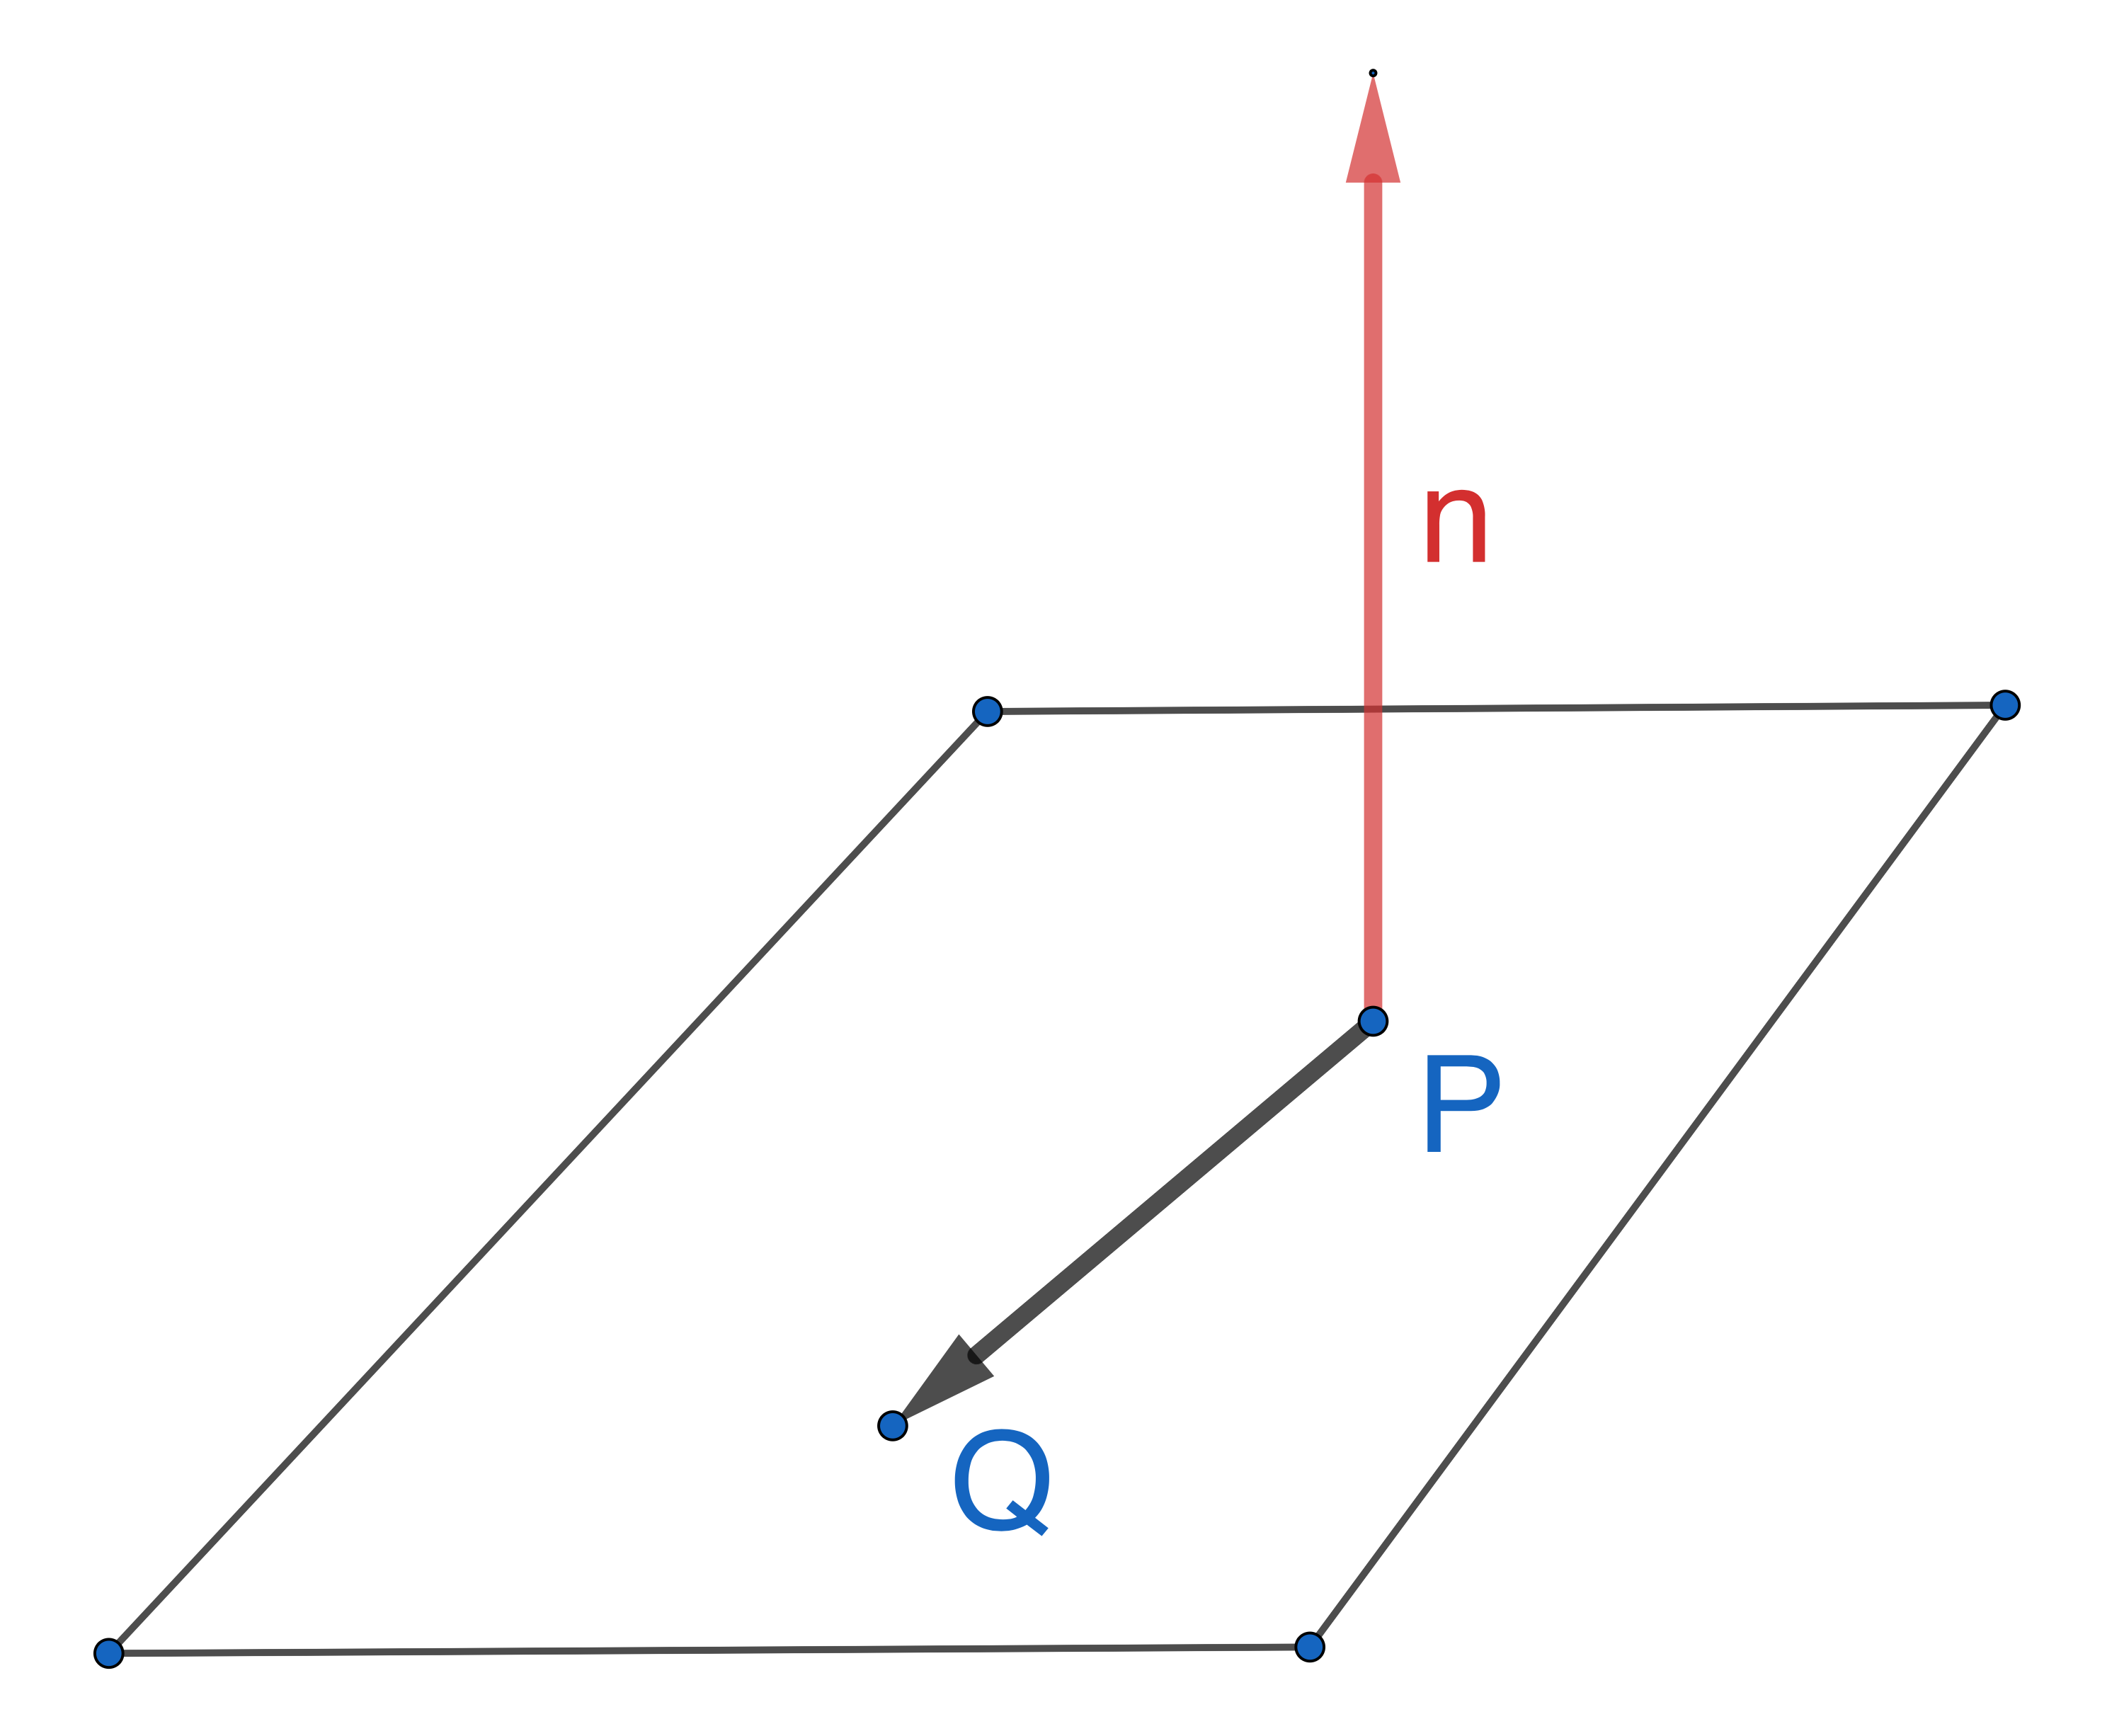
\includegraphics[scale=1]{normal-to-plane.png}
    \column{0.4\textwidth}
    \begin{itemize}
    \item Let $P$ and $n$ be vectors in $\mathbb{R}^3$.
    \item The set of points $Q$ such that $\overrightarrow {PQ}$ is orthogonal to $n$ form a plane.
    \item Therefore the solutions to
      \begin{equation*}
        n\cdot (x-P) = 0
      \end{equation*}
      form a plane through $P$ and orthogonal to $n$.
    \end{itemize}
  \end{columns}
\end{frame}

\begin{frame}{Examples}
  \begin{example}
    Find all vectors orthogonal to both
    \begin{equation*}
      \left[
	\begin{array}{c}
          -1\\
          -3\\
          2
	\end{array}
      \right]\text{ and }
      \left[
	\begin{array}{c}
          0\\
          1\\
          1
	\end{array}
      \right]
    \end{equation*}
  \end{example}
  \begin{example}
    Are the following the vertices of a right angled triangle?
    \begin{equation*}
      \left[
	\begin{array}{c}
          4\\
          -7\\
          9
	\end{array}
      \right], \left[
	\begin{array}{c}
          6\\
          4\\
          4
	\end{array}
      \right], \left[
	\begin{array}{c}
          7\\
          10\\
          -6
	\end{array}
      \right]
    \end{equation*}
  \end{example}
\end{frame}

\begin{frame}{Example}
  \begin{example}
    Find an equation of the plane containing
    \begin{equation*}
      \left[
	\begin{array}{c}
          1\\
          -1\\
          0
	\end{array}
      \right]
    \end{equation*}
    orthogonal to
    \begin{equation*}
      \left[
	\begin{array}{c}
          -3\\
          5\\
          2
	\end{array}
      \right]
    \end{equation*}
  \end{example}
  \begin{example}
    A rhombus is a parallelogram with sides of equal length.
    Prove that the diagonals of a rhombus are perpendicular.
  \end{example}
\end{frame}

\begin{frame}
  Questions?
\end{frame}

\section{Projections}

\begin{frame}
  \begin{beamercolorbox}[sep=12pt,center]{part title}
    \usebeamerfont{section title}\insertsection\par
  \end{beamercolorbox}
\end{frame}

\begin{frame}{Projection onto a vector}
  \begin{columns}
    \column{0.5\textwidth}
    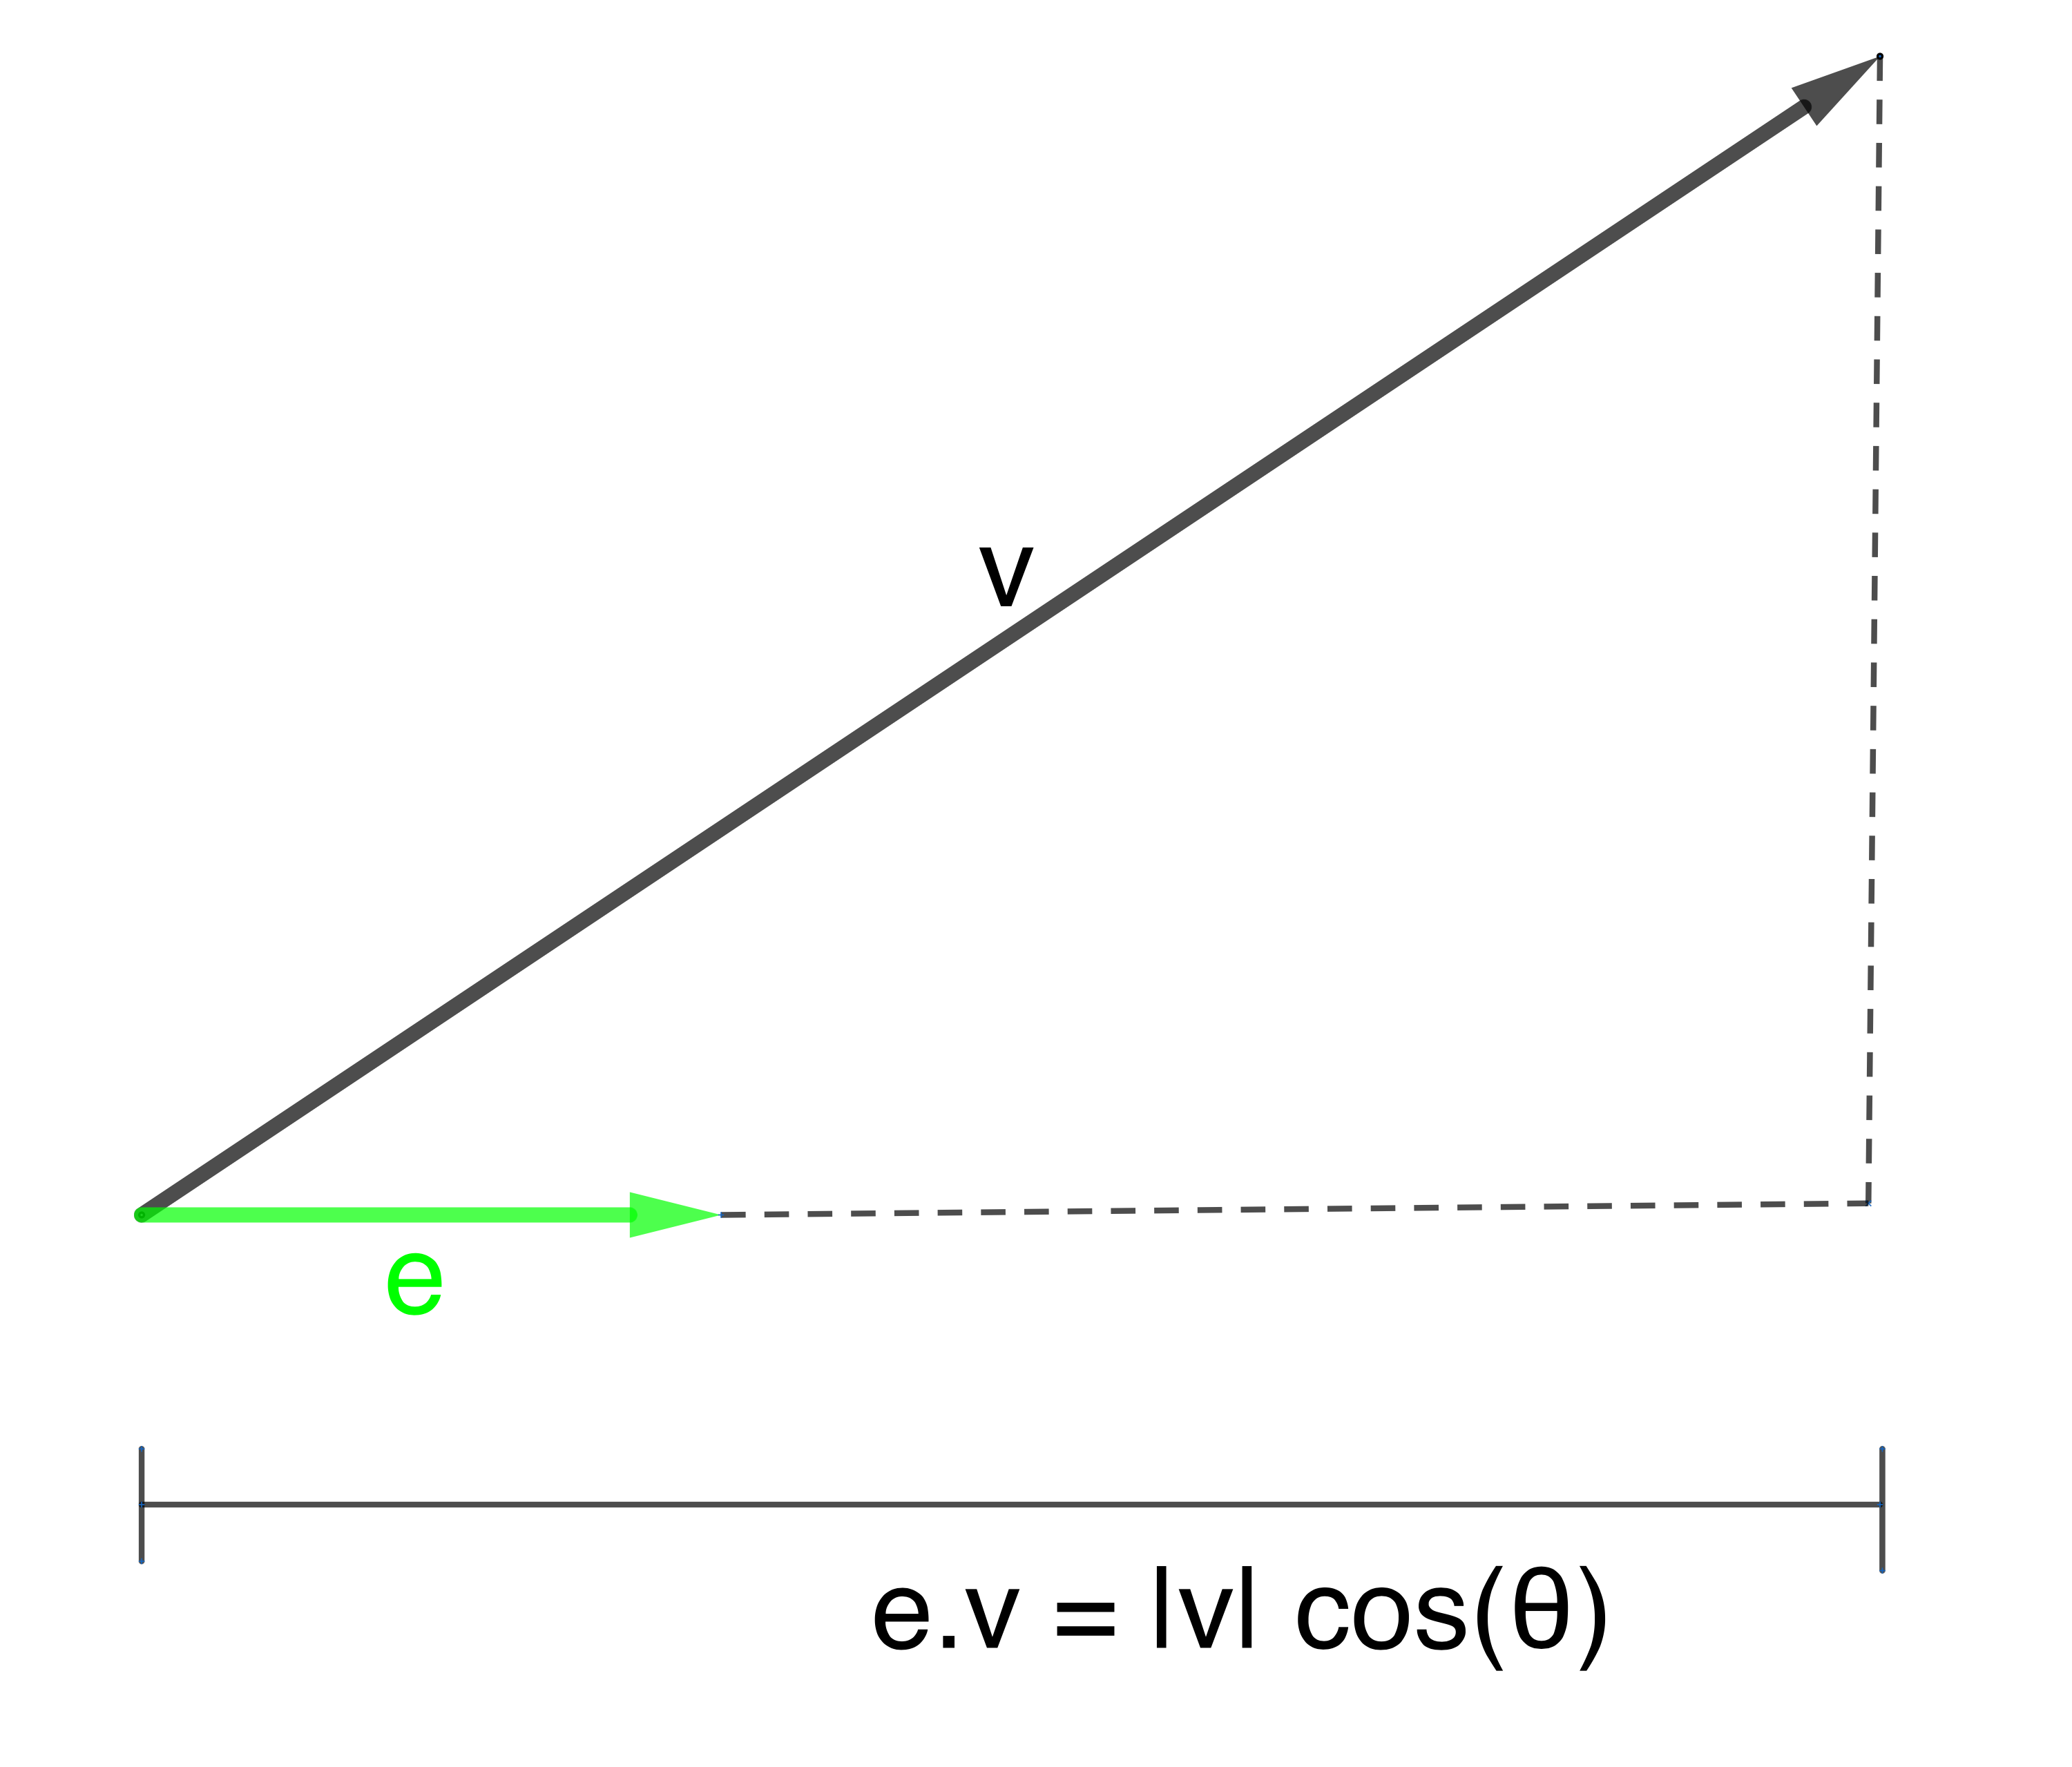
\includegraphics[scale=1.7]{projection-onto-unit.png}
    \column{0.4\textwidth}
    If $e$ is a unit vector then
    \begin{equation*}
      e\cdot v = |e||v|\cos \theta = |v|\cos \theta
    \end{equation*}
    and so $e\cdot v$ is the length of $v$ projected onto the line in direction $e$.
  \end{columns}
\end{frame}

\begin{frame}{Projection onto a vector}
  \begin{columns}
    \column{0.5\textwidth}
    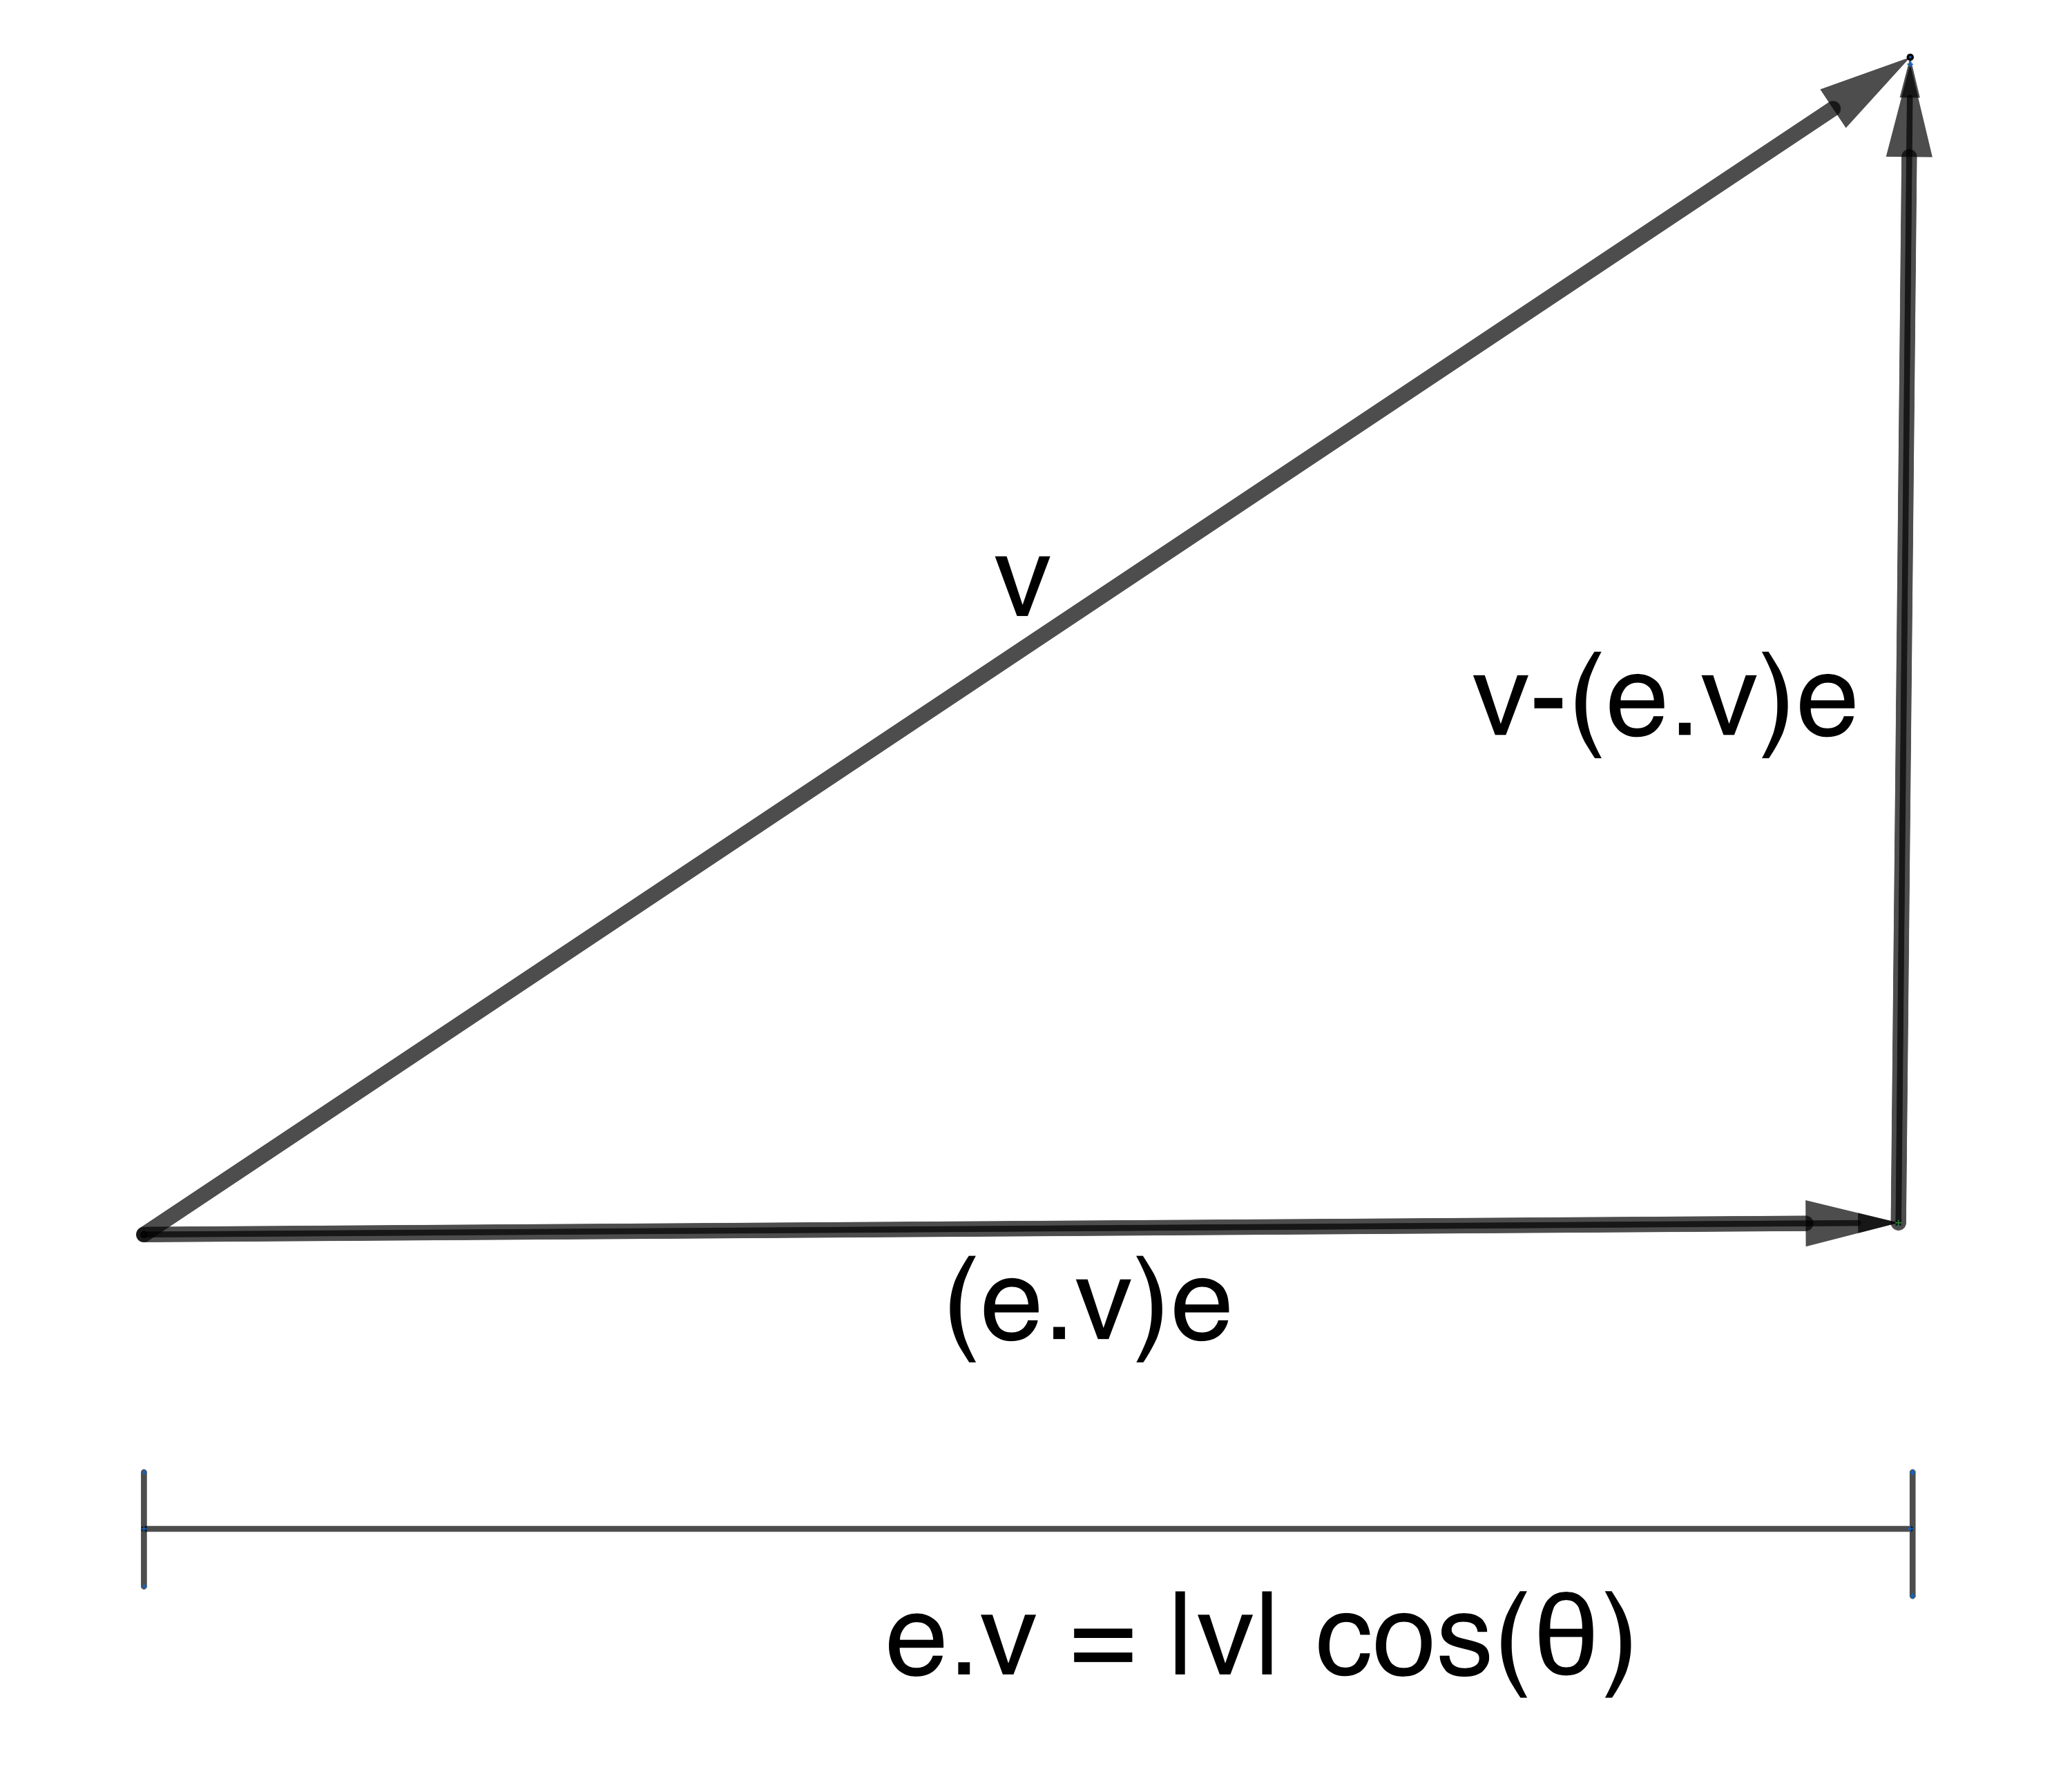
\includegraphics[scale=1.7]{decomposition-vector.png}
    \column{0.4\textwidth}
    Therefore we can write
    \begin{equation*}
      v = (e\cdot v)e + (v- e(e\cdot v))
    \end{equation*}
    where $(e\cdot v)e$ is parallel to $e$ and $(v- e(e\cdot v))$ is orthogonal to $e$.
  \end{columns}
\end{frame}

\begin{frame}{Examples}
  \begin{example}
    Let
    \begin{equation*}
      v = \left[
	\begin{array}{c}
          2\\
          -1\\
          0
	\end{array}
      \right]\text{ and }
      u = \left[
	\begin{array}{c}
          3\\
          1\\
          -1
	\end{array}
      \right]
    \end{equation*}
    Find vectors $v_0$ and $v_1$ such that $v = v_0 + v_1$, $v_0$ is orthogonal to $u$ and $v_1$ is parallel to $u$.
  \end{example}
\end{frame}

\begin{frame}
  Questions?
\end{frame}

\section{Closest points}

\begin{frame}
\begin{beamercolorbox}[sep=12pt,center]{part title}
\usebeamerfont{section title}
\insertsection\par
\end{beamercolorbox}
\end{frame}

\begin{frame}{Line given by parametric equations}
    \begin{columns}
        \hspace{-1cm}
        \column{0.5\textwidth}
        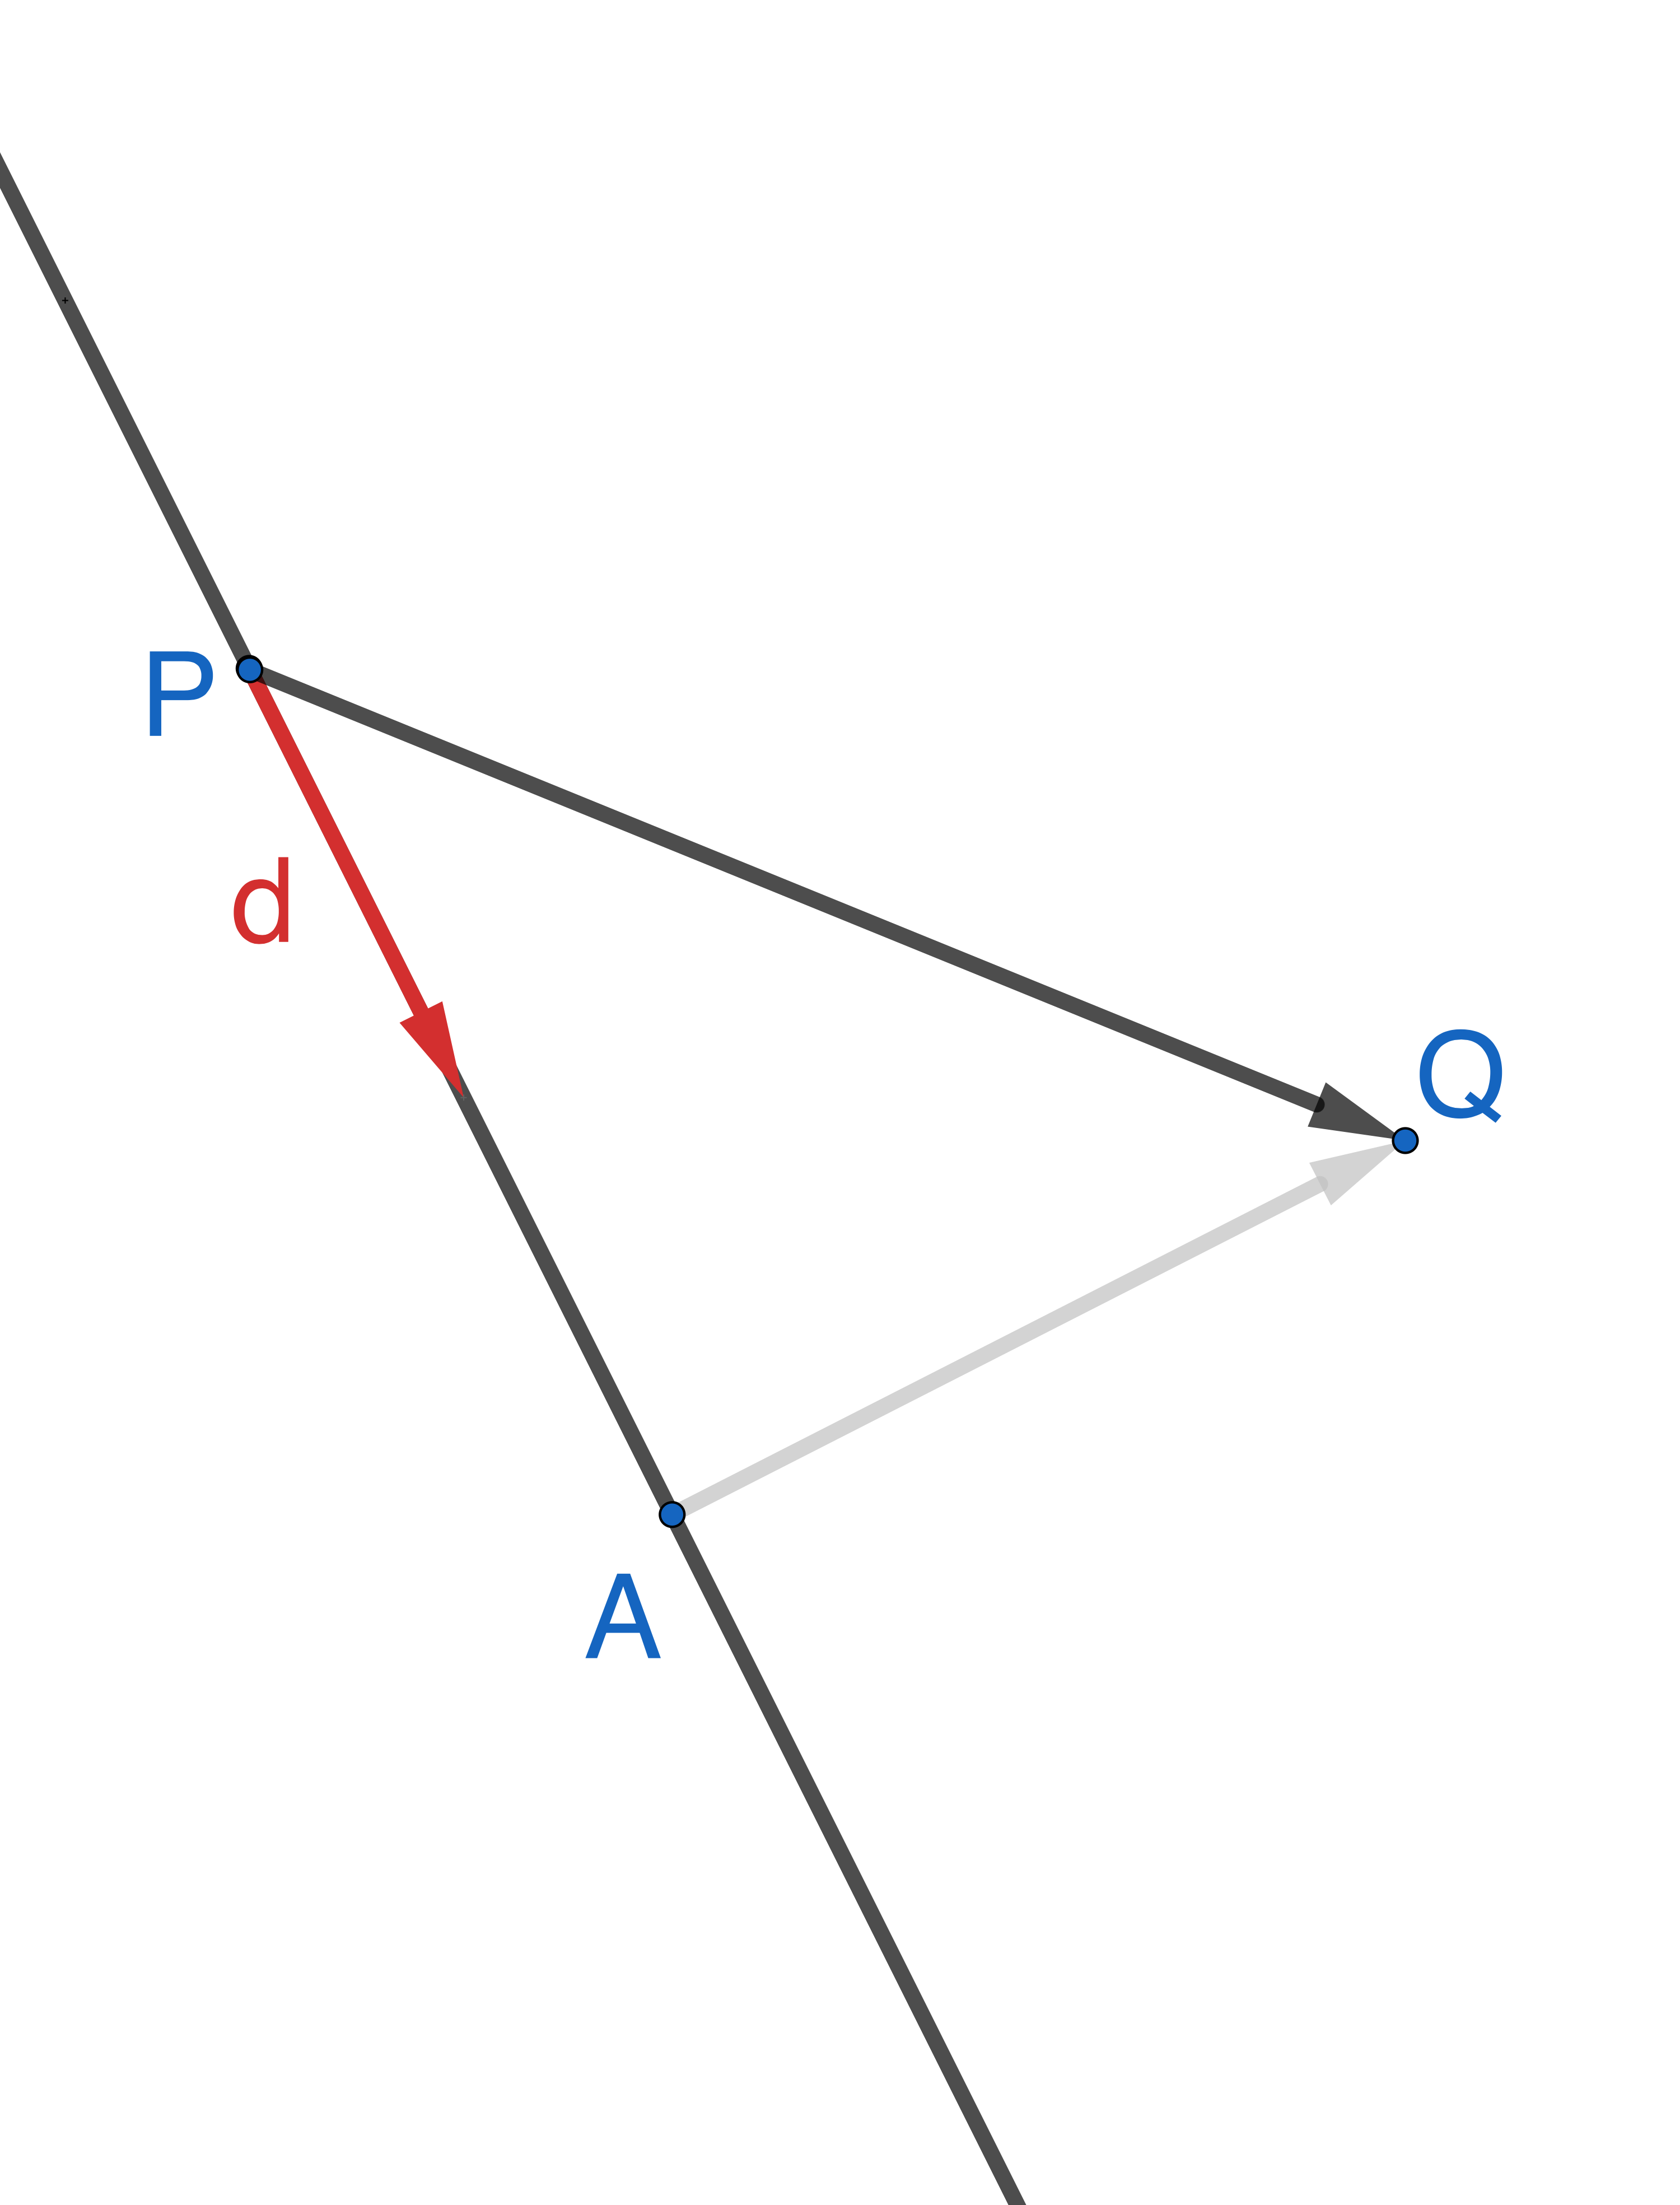
\includegraphics[scale=0.6]{2d-parametric-closest.png}
        \column{0.4\textwidth}
        First we project onto the direction of the line:
        \begin{equation*}
            \overrightarrow {PA} = \frac{d}{\|d\|}\cdot (Q-P)\frac{d}{\|d\|}
        \end{equation*}
        and then we can find $A$:
        \begin{equation*}
            A = P + \frac{d}{\|d\|}\cdot (Q-P)\frac{d}{\|d\|}
        \end{equation*}
        (Use same technique for line in $\mathbb R^n$ also.)
    \end{columns}
\end{frame}

\begin{frame}{Line given by normal}
\begin{columns}
    \hspace{-1cm}
    \column{0.5\textwidth}
    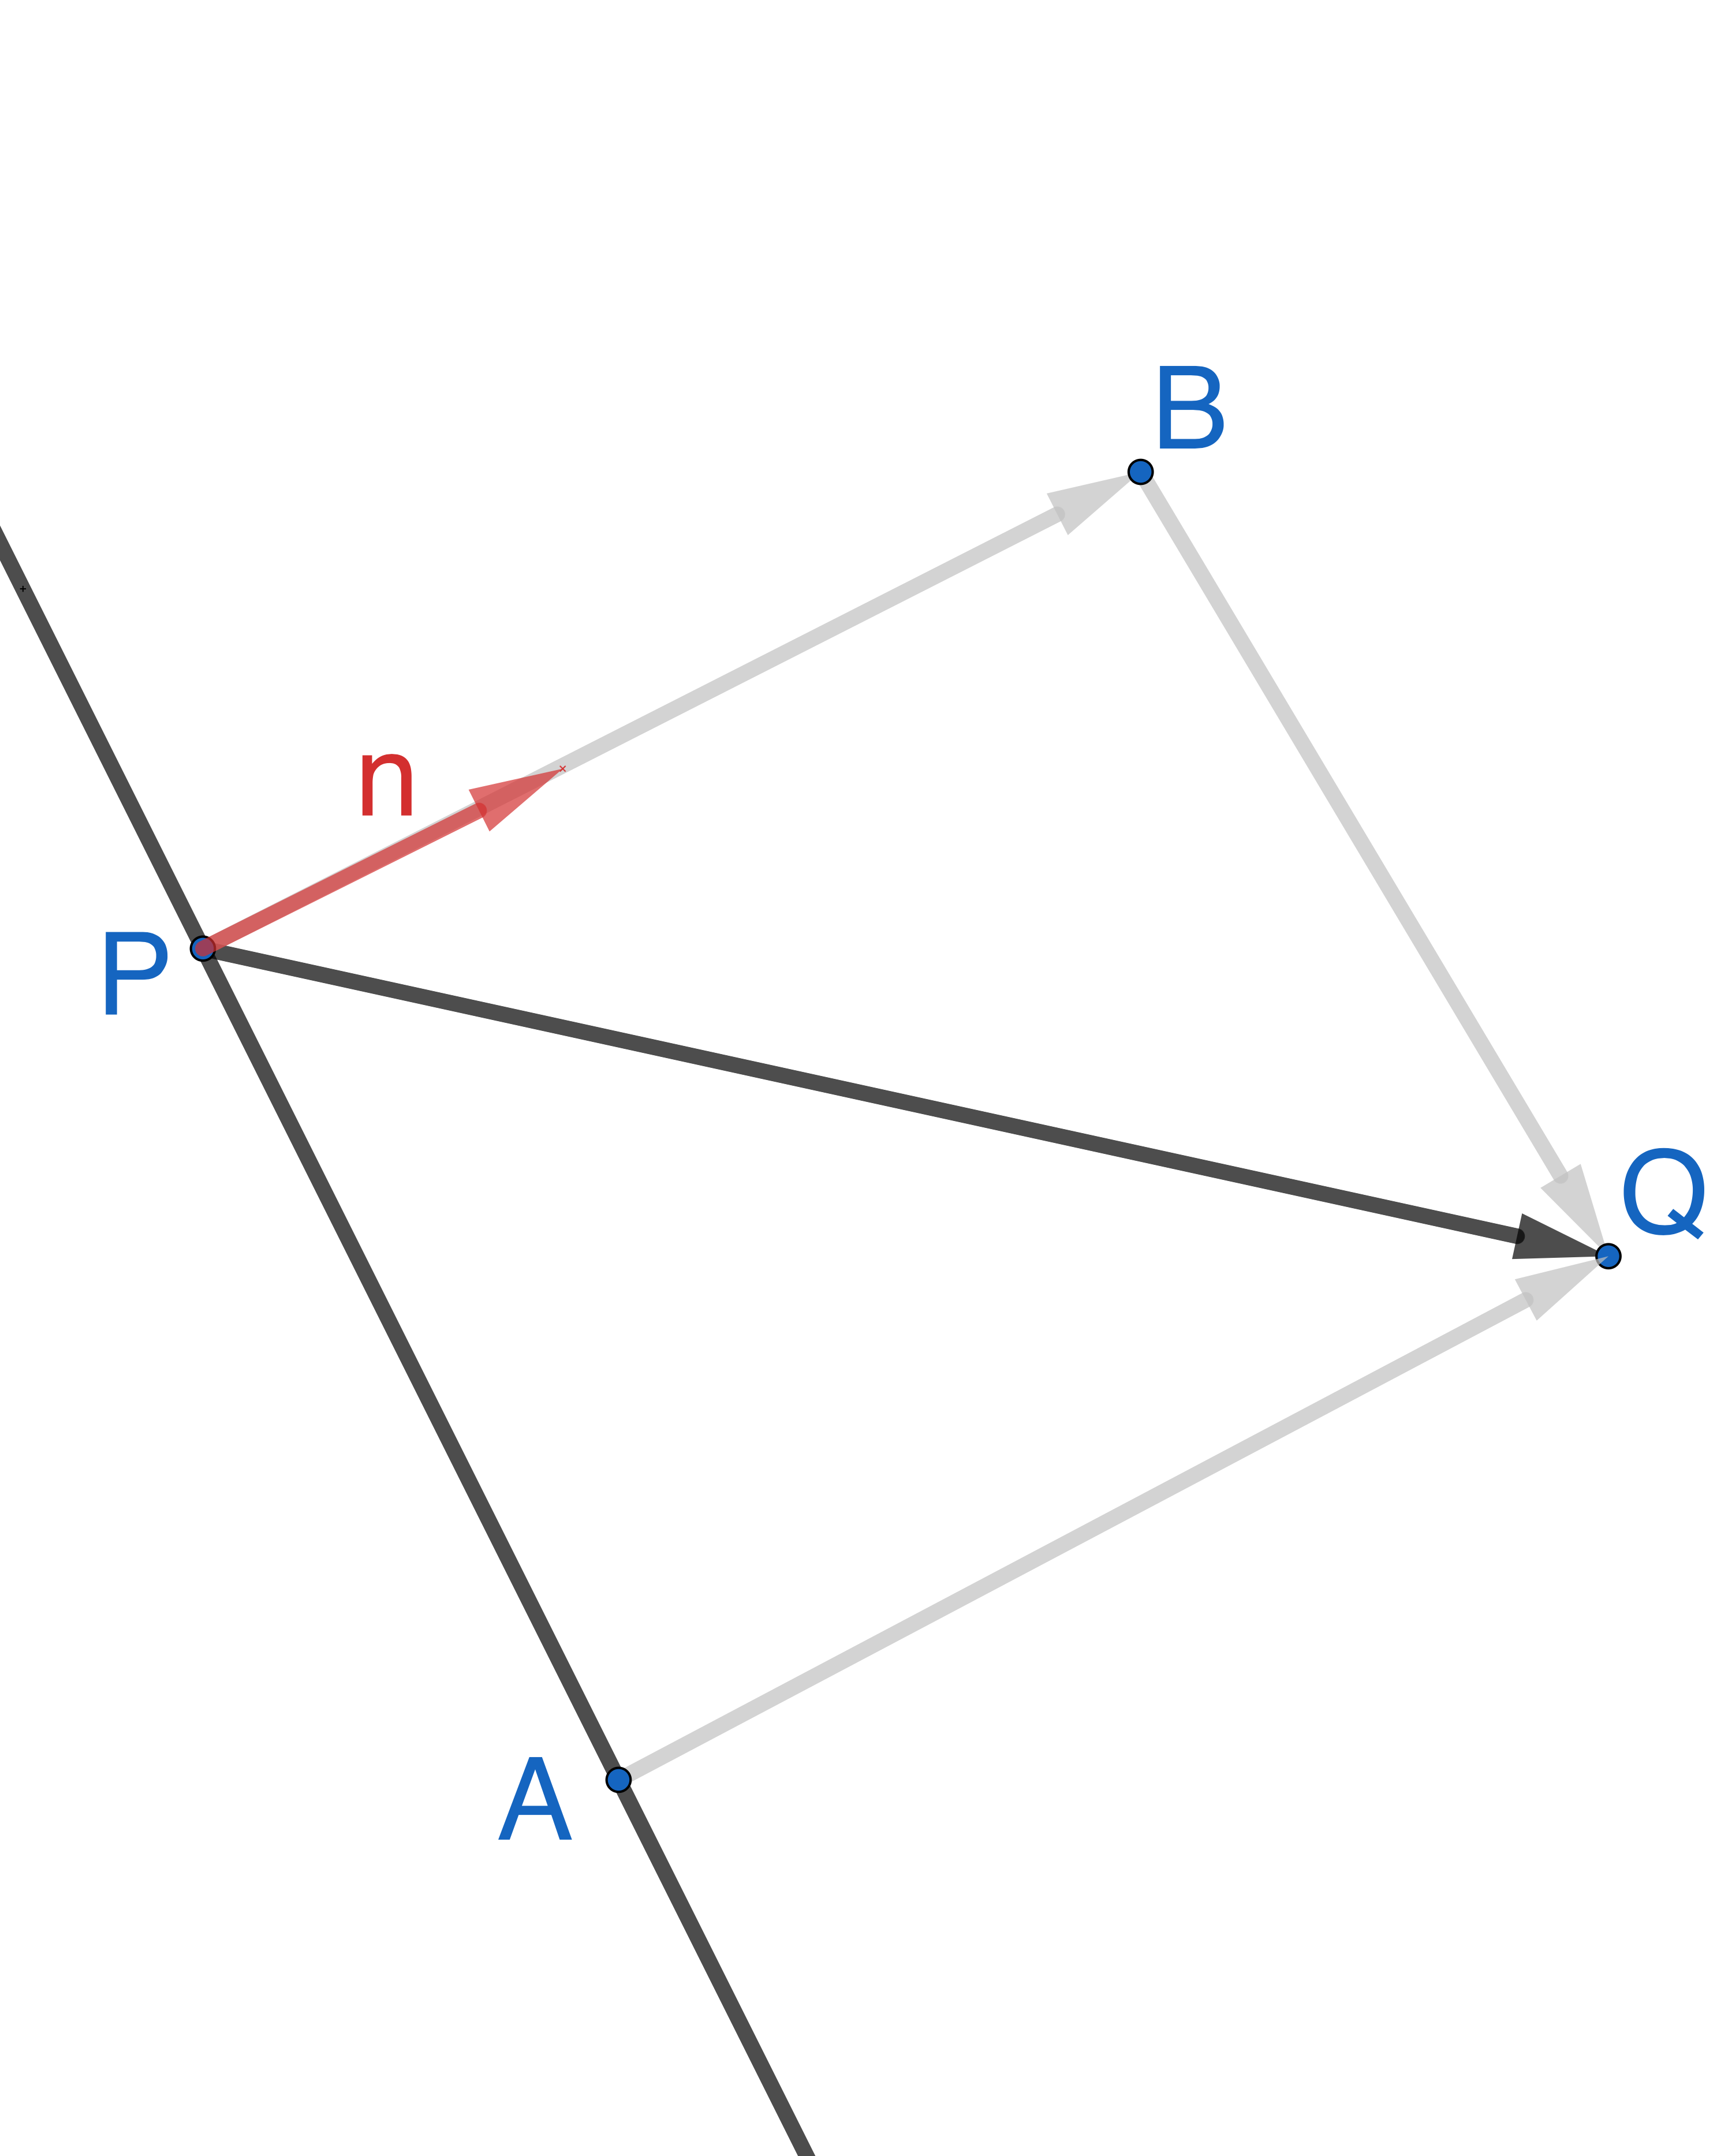
\includegraphics[scale=0.6]{2d-normal-closest.png}
    \column{0.4\textwidth}
    In this picture
    \[
        \overrightarrow{PB}\|\overrightarrow{AQ}\text{ and } \overrightarrow{PA}\| \overrightarrow{BQ}
    \]  
    First we project onto the normal:
    \begin{equation*}
        \overrightarrow {PB} = \frac{n}{\|n\|}\cdot (Q-P)\frac{n}{\|n\|}
    \end{equation*}
    and then we can find $A$:
    \begin{equation*}
        A = Q - \frac{n}{\|n\|}\cdot (Q-P)\frac{n}{\|n\|}
    \end{equation*}
    (Use same technique for $(n-1)$-dimensional hyperplane in $\mathbb R^n$ also.)
\end{columns}
\end{frame}

\begin{frame}{Example}
    \begin{example}
    If
    \begin{equation*}
      p= \left[
	\begin{array}{c}
          3\\
          2\\
          -1
	\end{array}
      \right]
    \end{equation*}
    find the closest point to $p$ on the following line:
    \begin{equation*}
      \left[
	\begin{array}{c}
          x_1\\
          x_2\\
          x_3
	\end{array}
      \right] = \left[
	\begin{array}{c}
          2\\
          1\\
          3
	\end{array}
      \right]+s \left[
	\begin{array}{c}
          3\\
          -1\\
          -2
	\end{array}
      \right]
    \end{equation*}
  \end{example}
\end{frame}

\begin{frame}{Example}
    \begin{example}
        Find the closest point to
        \begin{equation*}
          \left[
        \begin{array}{c}
              2\\
              3
        \end{array}
          \right]
        \end{equation*}
        on the line with equation $4x+3y = -2$.
      \end{example}
    \begin{example}
    Find the closest point to
    \begin{equation*}
      \left[
	\begin{array}{c}
          2\\
          3\\
          0
	\end{array}
      \right]
    \end{equation*}
    on the plane with equation $5x+y+z = -1$.
  \end{example}
\end{frame}

\section{Misc}

\begin{frame}
\begin{beamercolorbox}[sep=12pt,center]{part title}
\usebeamerfont{section title}
\insertsection\par
\end{beamercolorbox}
\end{frame}

\begin{frame}{Cauchy-Schwarz inequality}
\begin{columns}
    \hspace{-1cm}
    \column{0.5\textwidth}
    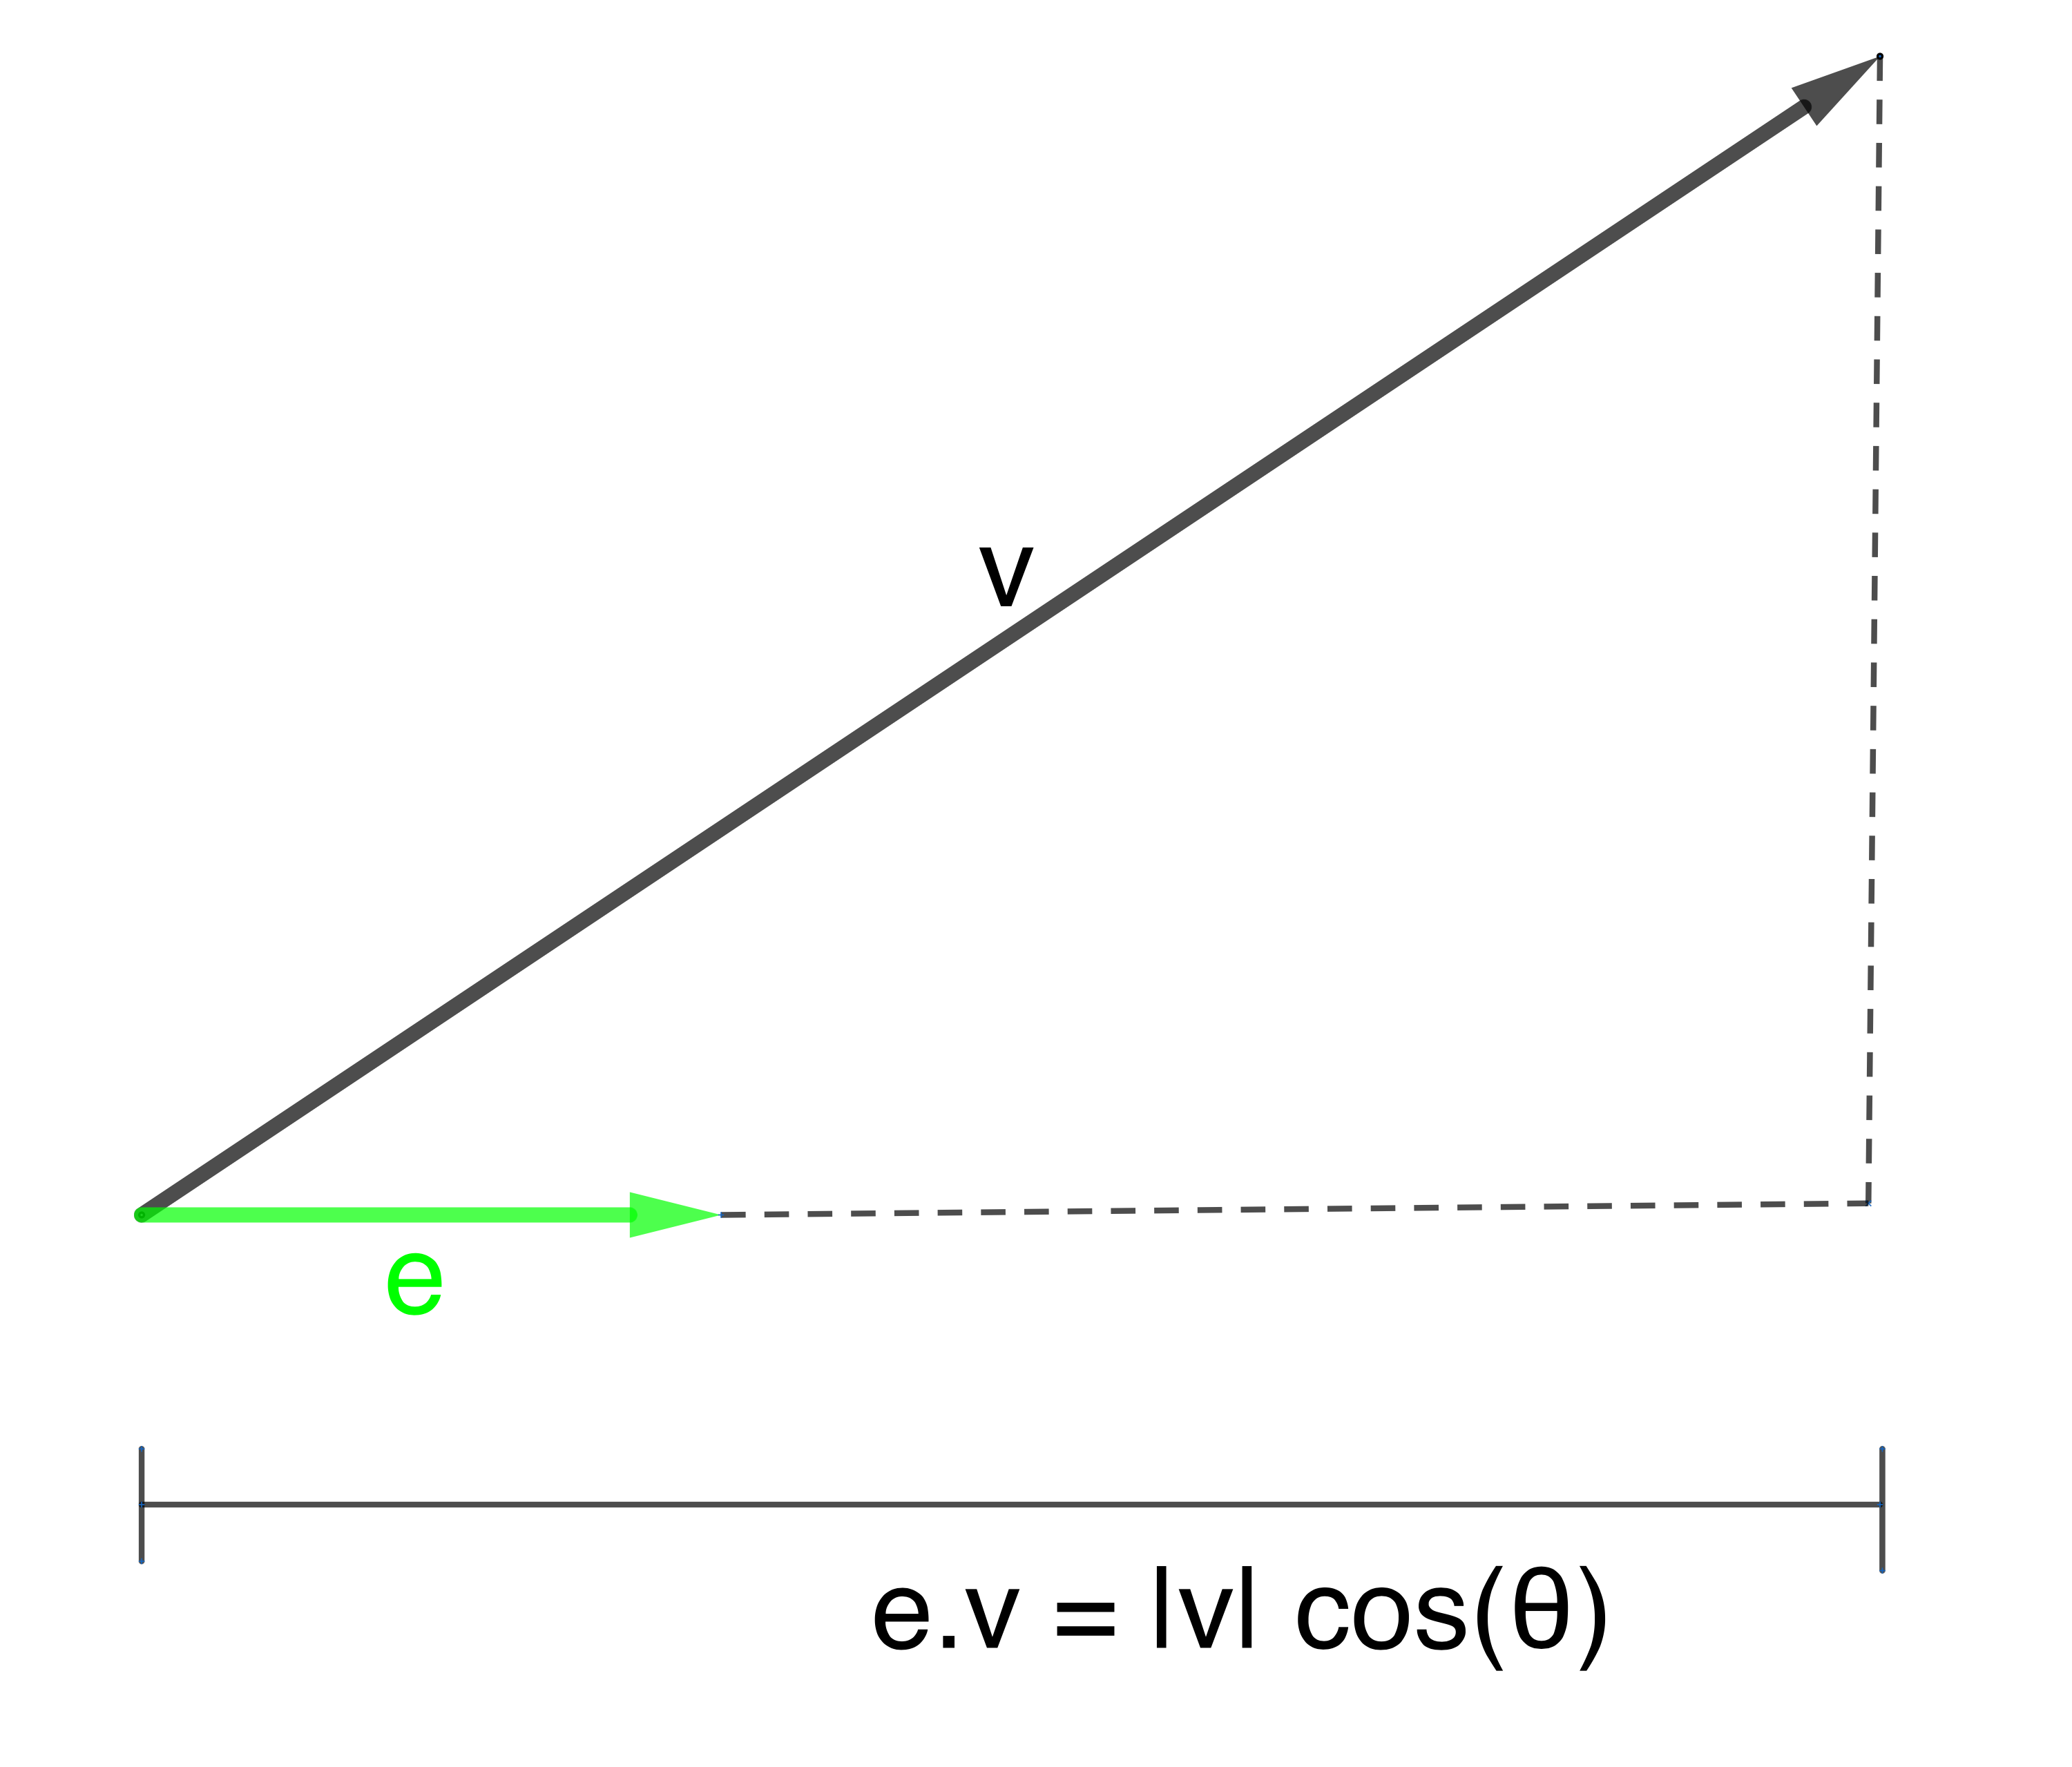
\includegraphics[scale=1.7]{projection-onto-unit.png}
    \column{0.45\textwidth}
    If $e$ is a unit vector then
    \begin{equation*}
    |e\cdot v| \leq \|v\|
    \end{equation*}
    More generally:
    \begin{equation*}
        |u\cdot v| \leq \|u\|\|v\|
    \end{equation*}
    which is the \emph{Cauchy-Schwarz inequality}.
\end{columns}
\end{frame}

\begin{frame}{Triangle inequality}
\begin{theorem}
  If $u$ and $v$ are vectors in $\mathbb{R}^n$ then
  \begin{equation*}
    \|u+v\| \leq \|u\|+\|v\|
  \end{equation*}
\end{theorem}\vfill
\begin{theorem}
  If $u$ and $v$ are vectors in $\mathbb{R}^n$ then
  \begin{equation*}
    |\|u\|-\|v\||\leq \|u-v\|
  \end{equation*}
\end{theorem}
\end{frame}

\begin{frame}{Example}
    \begin{example}
        Find equations for the lines through
        \begin{equation*}
            \left[
            \begin{array}{c}
            1\\
            0\\
            1
            \end{array}
            \right]
        \end{equation*}
        that meet the line
        \begin{equation*}
            \left[
            \begin{array}{c}
            x\\
            y\\
            z
            \end{array}
            \right] = \left[
            \begin{array}{c}
            1\\
            2\\
            0
            \end{array}
            \right]+s \left[
            \begin{array}{c}
            2\\
            -1\\
            2
            \end{array}
            \right]
        \end{equation*}
        at the two points distance three from $(1, 2, 0)$.
    \end{example}
\end{frame}

\begin{frame}{Examples}
    \begin{example}
        The diagonals of a parallelogram bisect each other.
      \end{example}
      \begin{example}
        If $ABCD$ is an arbitrary quadrilateral then the midpoints of the four sides form a parallelogram.
      \end{example}
\end{frame}

\end{document}